\documentclass[12pt%
%,draft%
,aspectratio=169%
]{beamer}
%
\usepackage{fontspec}
\defaultfontfeatures{Ligatures=TeX}
%\setsansfont{Liberation Sans}
\usepackage{polyglossia}
\setdefaultlanguage{ngerman}
% Alternative template for talks of the Freie Universität Berlin.
% Created by Leonard R. König, <leonard.koenig@fu-berlin.de> following the
% guidelines on www.fu-berlin.de/cd
%
% (c) Leonard König, CC BY 4.0
%
% This template was written against UTF-8 capable LaTeX engines, specifically
% LuaLaTeX.

% Trying to get rather close to the ppt/odp template:
%  http://www.fu-berlin.de/sites/cd/downloads_container/PowerPoint_Praesentation_Anleitung.pdf

%%% font styles
\setbeamerfont{frametitle}{series=\bfseries}
\setbeamerfont{footline}{series=\bfseries}
\setbeamerfont{headline}{series=\bfseries}
\setbeamerfont{alerted text}{series=\bfseries}
%%%

% colordefs
\definecolor{fu_darkblue}{RGB}{0,51,102}
\definecolor{fu_seablue}{RGB}{0,102,204}
\definecolor{fu_lightblue}{RGB}{204,214,224}
\definecolor{fu_green}{RGB}{153,204,0}
\definecolor{fu_lightgrey}{RGB}{128,128,128}
\definecolor{fu_grey}{RGB}{95,95,95}
%
\definecolor{fu_red}{RGB}{204, 0, 0} % red text (used by \alert)
%%% end colordefs

%%% colors
\setbeamercolor*{title}{fg=fu_darkblue}
\setbeamercolor*{subtitle}{fg=fu_seablue}
\setbeamercolor*{frametitle}{fg=fu_darkblue}
\setbeamercolor*{footline}{fg=fu_grey,bg=fu_lightblue}
\setbeamercolor*{headline}{fg=fu_grey}

\setbeamercolor*{normal text}{fg=black}
\setbeamercolor*{alerted text}{fg=fu_red}
\setbeamercolor*{example text}{fg=fu_green}
\setbeamercolor*{structure}{fg=fu_darkblue}

\setbeamercolor*{block title}{fg=white,bg=black!50}
\setbeamercolor*{block title alerted}{fg=white,bg=black!50}
\setbeamercolor*{block title example}{fg=white,bg=black!50}

\setbeamercolor*{block body}{bg=black!10}
\setbeamercolor*{block body alerted}{bg=black!10}
\setbeamercolor*{block body example}{bg=black!10}

\setbeamercolor{bibliography entry author}{fg=fu_darkblue}

\setbeamercolor{item}{fg=fu_darkblue}
\setbeamercolor{navigation symbols}{fg=fu_lightgrey,bg=fu_grey}
%%% end colors

%%% title page
% Display logo (if exists) and right next to it, put our title + subtitle
\defbeamertemplate*{title page}{fu_titlepage}
{%
	\hskip .3\textheight
	\begin{minipage}[.4\textheight]{\textwidth}
		\begin{minipage}[.4\textheight]{0.25\textwidth}
			\inserttitlegraphic
		\end{minipage}%
		\begin{minipage}[.4\textheight]{0.75\textwidth}
			\begin{beamercolorbox}{title}
				\usebeamerfont{title}\inserttitle\par%
			\end{beamercolorbox}
			\vfill
			\ifx\insertsubtitle
				\@empty%
			\else
				\begin{beamercolorbox}{subtitle}
					\usebeamerfont{subtitle}\insertsubtitle\par
				\end{beamercolorbox}
			\fi
		\end{minipage}
	\end{minipage}%
	\hskip .3\textheight
}
%%% end title page

%%% headline
% display title, author and institute on the left;
% logo on the right.
\newcommand{\headlinetext}
{%
	\inserttitle\\[0.3em]%
	\insertauthor, %
	\insertshortinstitute
}
\newlength{\headlinewidth}
\setlength{\headlinewidth}{\paperwidth}
\addtolength{\headlinewidth}{-2\marginparsep}
\setbeamertemplate{headline}
{%
	\begin{beamercolorbox}[wd=\paperwidth]{headline}%
		\vskip5pt
		{\hspace*{\marginparsep}}%
		\parbox{.5\headlinewidth}
		{%
			\usebeamertemplate{title in head/foot}%
			\headlinetext%
		}%
		\begin{minipage}{.5\headlinewidth}%
			\hfill\usebeamertemplate*{logo}
		\end{minipage}%
		{\hspace*{\marginparsep}}%
	\end{beamercolorbox}%
}
%%% end headline

%%% footline
% title + date on the left, frame number on the right
\newcommand{\footlinetext}
{%
	\usebeamerfont{shorttitle}\insertshorttitle, %
	\usebeamerfont{shortdate}\insertshortdate
}
\setbeamertemplate{footline}
{%
	\begin{beamercolorbox}{footline}
		\vskip2pt
		\hspace{\marginparsep}%
		\footlinetext\hfill%
		\insertframenumber%
		\hspace{\marginparsep}
		\vskip2pt
	\end{beamercolorbox}%
}
%%% end footline

% don't use default templates for sidebars
\setbeamertemplate{sidebar right}{}
\setbeamertemplate{sidebar left}{}
\setbeamertemplate{title page}[fu_titlepage]
\usepackage{amsmath}
\usepackage{amsfonts}
\usepackage{amssymb}
\usepackage{graphicx}
\usepackage{algorithm}
\usepackage[noend]{algpseudocode}
%\usepackage{algorithmic}
\usepackage{tikz}
\usetikzlibrary{arrows,shapes,automata,petri,positioning,calc}
\usepackage{graphicx}
\usepackage{subfig}
\usepackage{pgfplots}
\usepackage{venndiagram}
\usepackage{ stmaryrd }
\usepackage{circuitikz}
\usepackage{bohr}
\usepackage{csquotes}


\usepackage{luacode} % for '\luaexec' macro
%% Define a LaTeX "wrapper" macro:
\newcommand\bitwiseXOR[2]{\luaexec{tex.sprint((#1)~(#2))}}
\newcommand\bitwiseAND[2]{\luaexec{tex.sprint((#1)&(#2))}}
\newcommand\bitwiseOR[2]{\luaexec{tex.sprint((#1)|(#2))}}


\def\CalcC#1{%
\coordinate (base) at (#1.B);
\coordinate (collector) at (#1.C);
\coordinate (emitter) at (#1.E);
\draw (barycentric cs:base=0.32,collector=0.5,emitter=0.5) circle [radius=14pt];
}

\pgfplotsset{
    standard/.style={%Axis format configuration
        axis x line=middle,
        axis y line=middle,
        enlarge x limits=0.15,
        enlarge y limits=0.15,
        every axis x label/.style={at={(current axis.right of origin)},anchor=north west},
        every axis y label/.style={at={(current axis.above origin)},anchor=north east},
        every axis plot post/.style={mark options={fill=white}}
        }
    }


\author{Benjamin Tröster}
\title[Schalttechnik \& Logikgatter]{Schalttechnik \& Logikgatter}
%\subtitle[Markov Models]{...}
%\pgfdeclareimage{titlegraphic}{../res/dwarf_logo2.png}
%\titlegraphic{\pgfuseimage{titlegraphic}}
%\date{}
%\subject{}
%
% FU settings
\institute[HTW Berlin]{Hochschule für Technik und Wirtschaft Berlin}
%\pgfdeclareimage[height=0.9cm]{logo}{../res/dwarf_logo}
%\logo{\pgfuseimage{logo}}
%
\usepackage[
backend=biber,
citestyle=alphabetic,bibstyle=authoryear
]{biblatex}
\addbibresource{sources.bib}


\begin{document}

\begin{frame}
\titlepage
\end{frame}

\begin{frame}{Fahrplan}
\tableofcontents[hideothersubsections]
\end{frame}

\section{Recap}
\begin{frame}{Bool'sche Algebra nach Huntington (\textbf{Wichtig!})}
\begin{definition}
Die bool'sche Algebra nach Huntington ist definiert als Menge $\mathcal{V}: \{0,1\}$ mit den Verknüpfungen $\cdot (\land), + (\lor)$, sodass $\mathcal{V} \times \mathcal{V} \to \mathcal{V}$, also $\{0,1\} \times \{0,1\} \to \{0,1\}$. 
\end{definition}
\begin{itemize}
	\item Kommutativgesetze (K): $a \cdot b = b \cdot a$ bzw. $a + b = b + a$
	\item Distributivgesetze (D): $a \cdot (b + c) = (a \cdot b) + (a \cdot c)$ bzw. $a + (b \cdot c) = (a + b) \cdot (a + c)$
	\item Neutrale Elemente (N): $ \exists e, n \in \mathcal{V}$ mit  $a \cdot e = a$ und $a + n = a$
	\item Inverse Elemente (I): $\forall a \in \mathcal{V}$ existiert ein $a'$ mit $a \cdot a'= n$ und $a + a' = e$
\end{itemize}
Übernommen von \cite{barnett2013boolean} bzw. \cite{hoffmann2020grundlagen}
\end{frame}

\begin{frame}{Notation und Operatorenbindung}
\begin{itemize}
	\item Syntactic Sugar (Ableitungen aus Basisverknüpfungen)
	\begin{itemize}
		\item $(a \Rightarrow b)$ für $(\neg a \lor b)$ -- Implikation
		\item $(a \Leftarrow b)$ für $(b \Rightarrow a)$ -- Inversion der Implikation
		\item $(a \Leftrightarrow b)$ für $(a \Rightarrow b) \land (a \Leftarrow b)$ -- Äquivalenz
		\item $(a \oplus b)$ für $\neg (a \Leftrightarrow b)$ -- Antivalenz oder Exklusiv-ODER/XOR
		\item $\neg(a \lor b)$ -- NOR
		\item $\neg (a \land b)$ -- NAND
	\end{itemize}
	\item Bindung der Operatoren 
	\begin{itemize}
		\item $\land$ bindet stärker als $\lor$
		\item $\neg$ bindet stärker als $\land$
	\end{itemize}
	\item Klammerung
	\begin{itemize}
		\item Gleiche Verknüpfungen: linksassoziativ zusammengefasst
	\end{itemize}
\end{itemize}	 
\end{frame}

\begin{frame}{Erfüllbarkeit}
	\begin{definition}[Erfüllbarkeit]
		Sei $\varphi$ ein beliebiger boolescher Ausdruck. $\varphi$ heißt
		\begin{itemize}
			\item erfüllbar, wenn es Werte $x_1, \ldots, x_n$ gibt, mit $\varphi (x_1, \ldots, x_n ) = 1$.
			\item widerlegbar, wenn es Werte $x_1, \ldots, x_n$ gibt, mit $\varphi (x_1, \ldots, x_n) = 0$.
			\item unerfüllbar, wenn $\varphi (x_1 ,\ldots , x_n )$ immer gleich $0$ ist.
			\item allgemeingültig, wenn wenn $\varphi (x_1 ,\ldots , x_n )$ immer gleich $1$ ist.
		\end{itemize}
		Einen allgemeingültigen Ausdruck bezeichnen wir auch als \textbf{Tautologie}.
	\end{definition}
\end{frame}


\begin{frame}{Negationstheorem}
\begin{theorem}[Negationstheorem]
Sei $f(0, 1, x_1 , \ldots , x_n , \land, \lor, \neg)$ ein boolescher Ausdruck, in dem neben den Konstanten $1$ und $0$ und den Variablen $x_1 ,\ldots, x_n$ die booleschen Operatoren $\land, \lor$ und $\neg$ vorkommen. Dann gilt:
$$
	\overline{f(0, 1, x_1 , \ldots , x_n , \land, \lor, \neg)} = f(1, 0, \overline{x_1}, \ldots ,\overline{x_n} ,\lor, \land, \neg)
$$
\end{theorem}
\end{frame}

\begin{frame}{Dualitätsprinzip}
\begin{theorem}
Sei
$$
\varphi(0, 1, x_1 , \ldots, x_n , \land, \lor, \neg) = \psi(0, 1, x_1 , \ldots, x_n , \land, \lor, \neg)
$$
ein Gesetz der booleschen Algebra, in der neben Variablen und den Konstanten $0$ und $1$ ausschließlich die Elementarverknüpfungen $\neg, \land$ und $\lor$ vorkommen. Dann ist auch die duale Gleichung
$$
\varphi(0, 1, x_1 , \ldots, x_n , \land, \lor, \neg) = \psi(0, 1, x_1 , \ldots, x_n , \land, \lor, \neg)
$$
ein Gesetz der booleschen Algebra.
\end{theorem}
\end{frame}

\begin{frame}{Vollständige Operatorensysteme}
\begin{definition}[Vollständige Operatorensystem]
$\mathcal{M}$ sei eine beliebige Menge von Operatoren. $\mathcal{M}$ ist ein vollständiges Operatorensystem, wenn sich jede boolesche Funktion durch einen Ausdruck beschreiben lässt, in dem neben den Variablen $x_1 , \ldots , x_n$ ausschließlich Operatoren aus $\mathcal{M}$ vorkommen.
\end{definition}
\begin{itemize}
	\item Die Elementaroperatoren $\land, \lor$ und $\neg$ bilden zusammen ein vollständiges Operatorensystem
	\item Die Operatoren NAND und NOR bilden jeder für sich bereits ein vollständiges Operatorensystem
	\item Die Implikation und die $0$ bilden zusammen ebenfalls ein vollständiges Operatorensystem
\end{itemize}
\end{frame}

\begin{frame}{Normalformdarstellungen}
\begin{itemize}
	\item Normalform beschreibt eine eindeutige Darstellung
	\item Vollform: Ausdruck, in dem jede Variable genau einmal vorkommt 
	\item Literal: Teilausdruck, der entweder negierte oder unnegierte Variable darstellt
	\item Wahrheitstafeldarstellung ist eine Art der Normalformdarstellungen
	\item Bool'sche Ausdrücke hingegen sind keine Normalformdarstellung
	\begin{itemize}
		\item Jede bool'sche Funktion durch unendlich viele Ausdrücke beschrieben werden
	\end{itemize}
\end{itemize}
\end{frame}

\begin{frame}{Disjunktive Normalform}
\begin{itemize}
	\item Die disjunktive Normalform (DNF) ist jene Darstellungsart, bei der eine Reihe von Vollkonjunktionen disjunktiv verknüpft wird. Negationen  treten nur in atomarer Form auf.
	\begin{itemize}
		\item $(A \land \neg B \land C) \lor (A \land B \land C) \lor (\neg A \land \neg B \land C)$ 
	\end{itemize}
	\item \item Die konjunktive Normalform (KNF) ist jene Darstellungsart, bei der eine Reihe von Volldisjunktionen konjunktiv verknüpft wird. Negationen treten nur in atomarer Form auf.
	\begin{itemize}
		\item $(\neg A \lor \neg B \lor \neg C) \land (A \lor B \lor C) \land (A \lor \neg B \lor \neg C)$ 
	\end{itemize}
	\item Andere Bezeichnungen:
	\begin{itemize}
		\item Kanonische disjunktive/konjunktive Normalform (KDNF/KKNF)
		\item Vollständige disjunktive/konjunktive Normalform
	\end{itemize}
\end{itemize}
\end{frame}

\begin{frame}{Bitweise logische Operationen}
\begin{center}
$A,B$ seien Bitvektoren, $\circ$ eine beliebige Verknüpfung
\begin{figure}
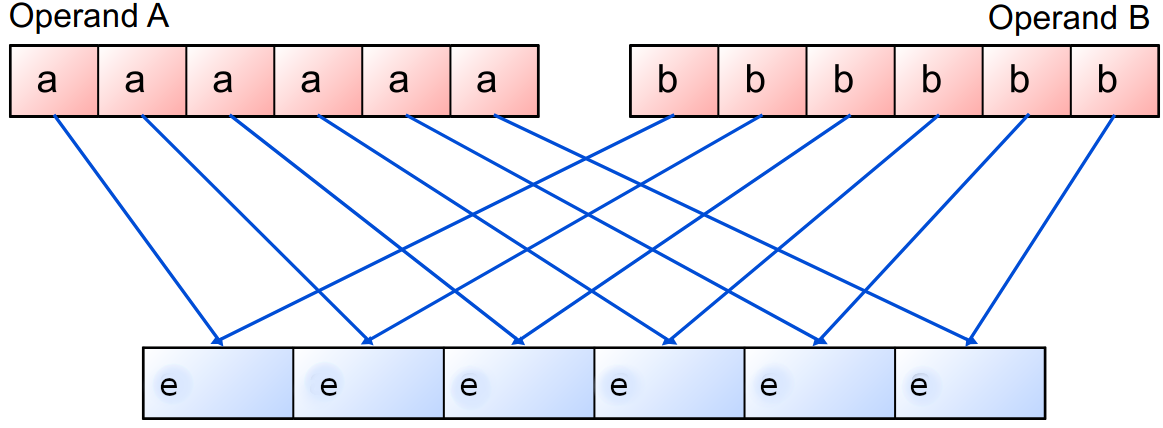
\includegraphics[scale=0.3]{pictures/bitvec}
\end{figure}
Dann erhalten wir als Ergebnis: $E = A \circ B$
\end{center}
\end{frame}

\section{Einleitung}
\begin{frame}{Heute:}
\begin{itemize}
	\item Von der Bool'schen Algebra zu Logikgattern
	\item Logische Schaltung auf Mikroprozessoren
	\item Idee der Arithmetic Logic Unit (also Co-Prozessor oder integriert)
	\item Grundlegende Logikgatter
	\item Grundlagen Leiter und Halbleiter
	\item Aufbau Transistor
	\item Transistortypen: Biopolar- und Feldeffekttransistor
	\item Vom Transistor zur logischen Schaltung
\end{itemize}
\end{frame}
\subsection{Beispiele}
\begin{frame}
	\begin{itemize}
		\item Status: Wir wissen, wie ein Signal von Analog auf Digital gewandelt wird
		\begin{itemize}
			\item Gist: wie kommen die Bits in den Rechner
		\end{itemize}
		\item Wir wissen, wie logische Aussagen verarbeitet werden können
		\item Noch offen: Wie werden hieraus komplexe Recheneinheiten?
		\begin{itemize}
			\item Erster Schritt wie können Elementarschaltungen realisiert werden
		\end{itemize}
	\end{itemize}
\end{frame}

\begin{frame}{Intel 4004 Prozessor}
\begin{figure}
\center
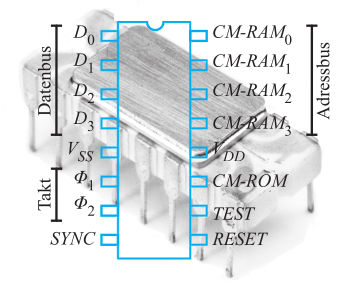
\includegraphics[scale=0.7]{pictures/4004}
\end{figure}
\end{frame}

\begin{frame}{Intel 4004 Prozessor}
\begin{figure}
\center
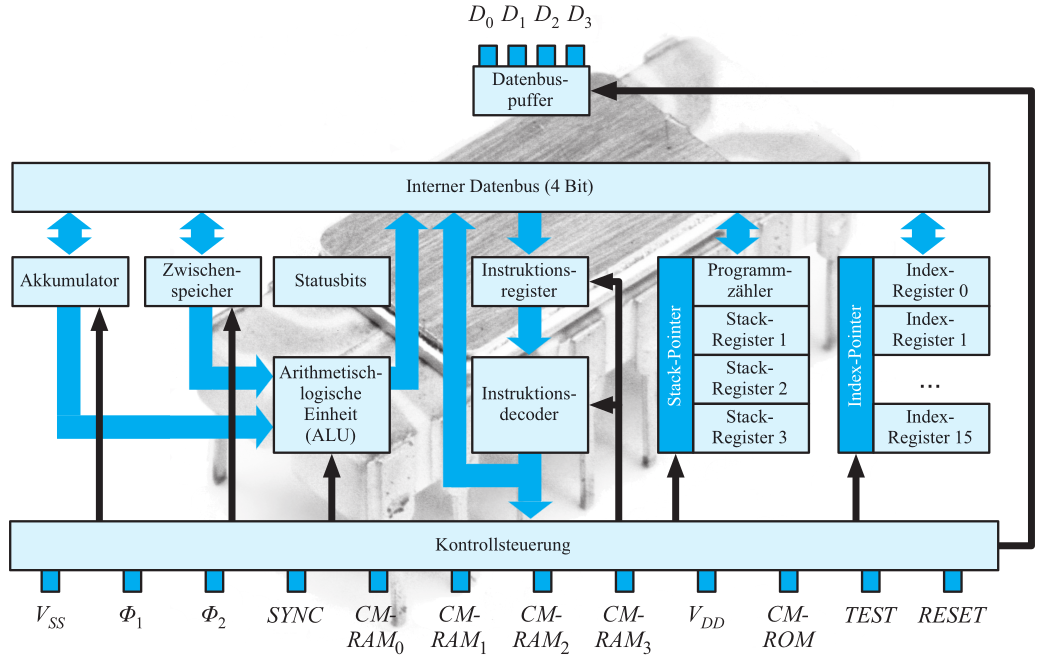
\includegraphics[scale=0.25]{pictures/4004_2}
\end{figure}
\end{frame}

\begin{frame}{4 Bit ALU Package Layout}
\begin{figure}
\center
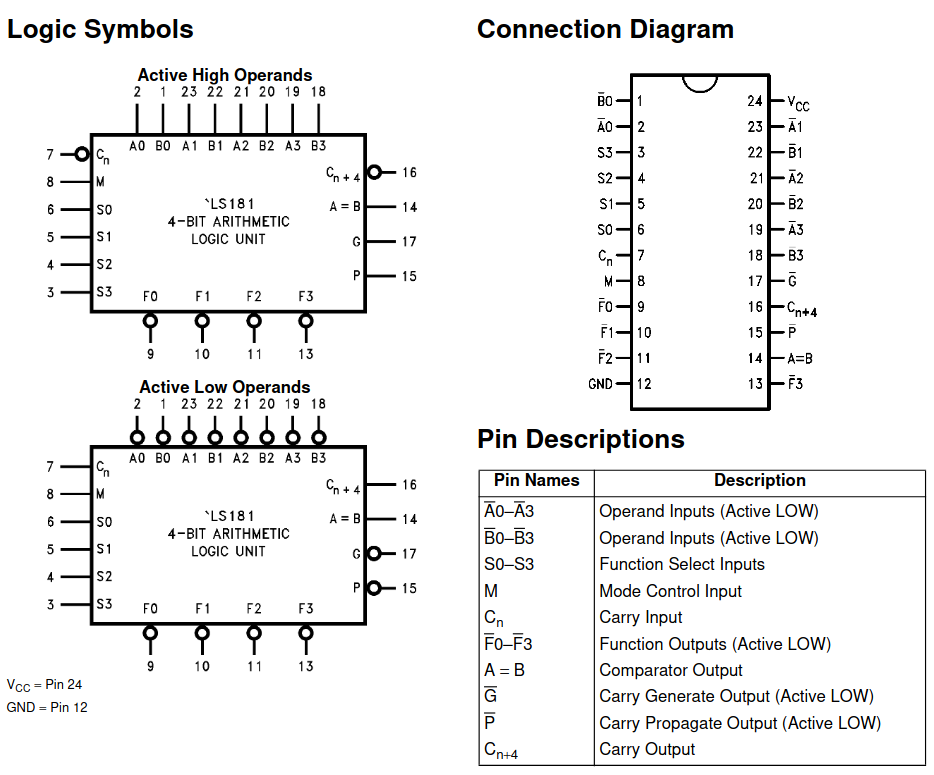
\includegraphics[scale=0.25]{pictures/layout_alu}
\end{figure}
\end{frame}


\begin{frame}{4 Bit ALU -- Logikgatter}
\begin{columns}[T] % align columns
\begin{column}{.48\textwidth}
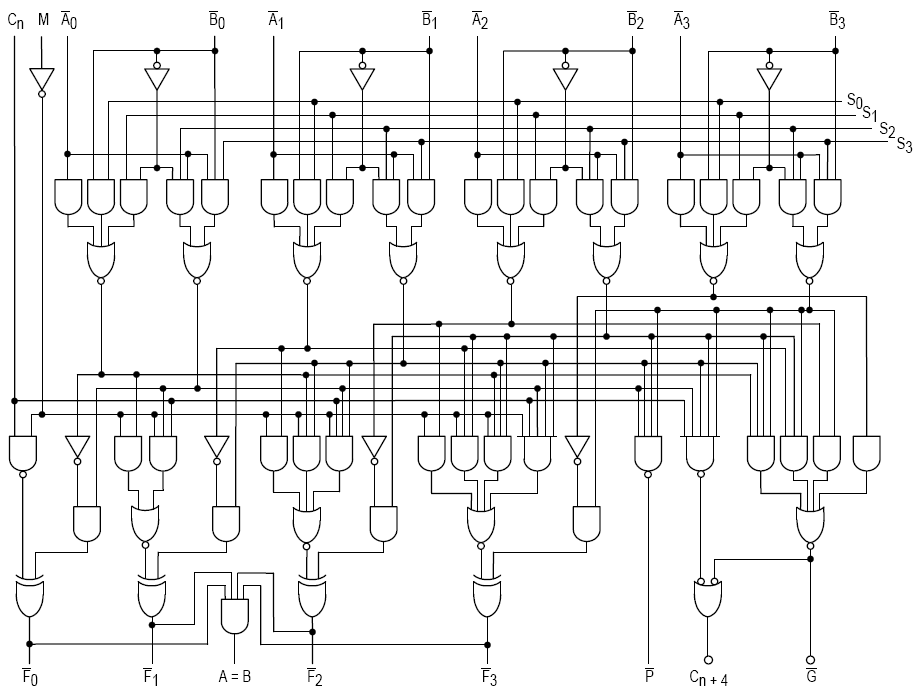
\includegraphics[scale=0.25]{pictures/alu2}
\end{column}%
\hfill%
\begin{column}{.48\textwidth}
\centering
\vspace*{1cm}
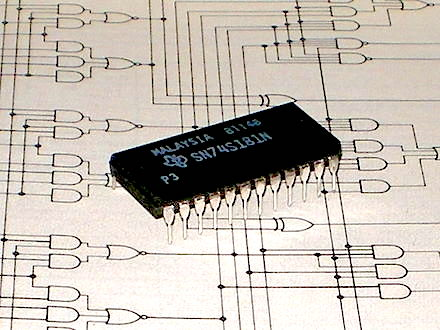
\includegraphics[scale=0.4]{pictures/alu1}
\end{column}%
\end{columns}
\end{frame}

\section{Bool'sche Algebra $\to$ Logikgatter}
\begin{frame}{Bool'sche Algebra $\to$ Logikgatter}
\begin{itemize}
	\item Bis jetzt abstrakt -- mathematische Definition der logischen Aussage
	\item D.h. Zuordnung von Werten auf binärer Ebene
	\item Umsetzung der bool'schen Funktionen mithilfe von Logikgattern (Gatter)	
	\item Physikalische Umsetzung beispielsweise mithilfe von Transistoren
\end{itemize}
\end{frame}

\begin{frame}{Darstellung Logikgatter}
\begin{figure}
\center
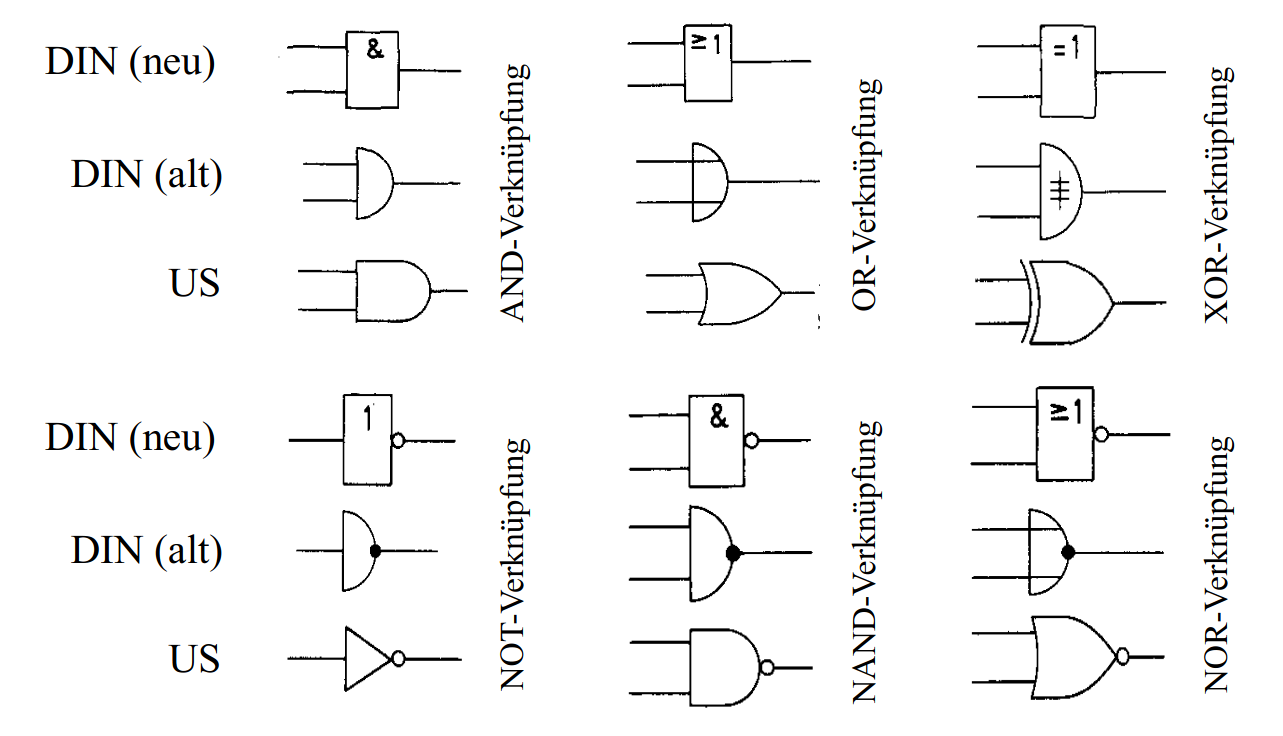
\includegraphics[scale=0.25]{pictures/logikgatter}
\end{figure}
\end{frame}


\begin{frame}{Beispiel: Paritätsfunktion}
\begin{columns}[T] % align columns
\begin{column}{.48\textwidth}
\vspace*{-1.5cm}
\begin{itemize}
	\item Eingänge: $x_1, x_2, x_3, x_4$
	\item Ausgänge: $y$
	\item Gatter: $XOR$
	\item Stufen: $2$
\end{itemize}

\end{column}%
\hfill%
\begin{column}{.48\textwidth}
\begin{circuitikz} 
\draw
(2,0) node[xor port] (xor1) {}
(2,2) node[xor port] (xor2) {}
(4,1) node[xor port] (xor3) {}
(xor1.in 1) node[left](f) {$X_3$}
(xor1.in 2) node[left](f) {$X_4$}
(xor2.in 1) node[left](f) {$X_1$}
(xor2.in 2) node[left](f) {$X_2$}
(xor1.out) |- (xor3.in 2)
(xor2.out) |- (xor3.in 1)
(xor3.out) node[right](j) {$y$};
;
\end{circuitikz}
\end{column}%
\end{columns}
\end{frame}


\begin{frame}{Beispiel: Paritätsfunktion}
\begin{columns}[T] % align columns
\begin{column}{.48\textwidth}
\begin{itemize}
	\item Eingänge: $x_1, x_2, x_3, x_4$
	\item Ausgänge: $y$
	\item Gatter: $XOR$
	\item Stufen: $2$
\end{itemize}
\begin{table}[]
\begin{tabular}{|l|l|l|l||l|}\hline
$x_1$ & $x_2$ & $x_3$ & $x_4$ & $y$ \\ \hline
0 & 0 & 0 & 0 & 0 \\ \hline
0 & 0 & 0 & 1 & 1 \\ \hline
0 & 0 & 1 & 0 & 1 \\ \hline
0 & 0 & 1 & 1 & 0 \\ \hline
0 & 1 & 0 & 0 & 1 \\ \hline
... & & & & \\ \hline
\end{tabular}
\end{table}
\end{column}%
\hfill%
\begin{column}{.48\textwidth}
\begin{circuitikz} 
\draw
(2,0) node[xor port] (xor1) {}
(2,2) node[xor port] (xor2) {}
(4,1) node[xor port] (xor3) {}
(xor1.in 1) node[left](f) {$X_3$}
(xor1.in 2) node[left](f) {$X_4$}
(xor2.in 1) node[left](f) {$X_1$}
(xor2.in 2) node[left](f) {$X_2$}
(xor1.out) |- (xor3.in 2)
(xor2.out) |- (xor3.in 1)
(xor3.out) node[right](j) {$y$};
;
\end{circuitikz}
\end{column}%
\end{columns}
\end{frame}

\section{Grundlagen}

\begin{frame}{Atommodell nach Bohr}
\begin{columns}[T] % align columns
\begin{column}{.48\textwidth}
\begin{itemize}
	\item Grundsätzlich: Kern -- Neutronen, Protonen
	\item Elektronen außerhalb des Kerns, frei beweglich in Orbitalräumen
	\item Äußerste Schale: Valenzelektronen
	%\item Valenzband zwischen äußerten Schale und 
	\item Zusammenschluss von Atomen über die Valenzelektronen
\end{itemize}
\end{column}%
\hfill%
\begin{column}{.48\textwidth}
\bohr{1}{H}
\bohr{2}{He}
\bohr{14}{Si}
\end{column}%
\end{columns}
\end{frame}

\subsection{Leiter \& Bändermodell}
\begin{frame}{Leiter \& Bändermodell}
\begin{columns}[T] % align columns
\begin{column}{.48\textwidth}
\vspace*{-0.2cm}
\begin{figure}
\center
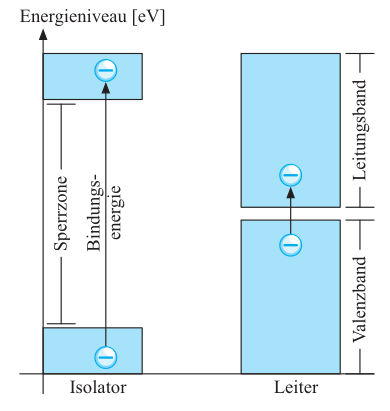
\includegraphics[scale=.45]{pictures/baendermod}
\end{figure}
\end{column}%
\hfill%
\begin{column}{.48\textwidth}
\vspace*{-0.3cm}
\begin{figure}
\center
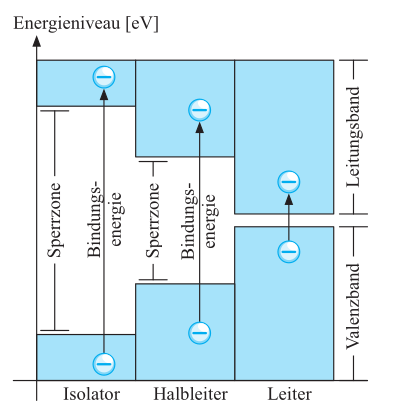
\includegraphics[scale=.45]{pictures/halbleiter_band}
\end{figure}
\end{column}%
\end{columns}
\end{frame}

\begin{frame}{Siliziumgitter}
\begin{columns}[T] % align columns
\begin{column}{.48\textwidth}
\begin{itemize}
	\item Struktur des Siliziumkristalls
	\item Jedes Atom ist von 4 weiteren Atomen umgeben
	\item Jeweils zwei gemeinsam genutzte Valenzelektronen eine stabile Verbindung
\end{itemize}
\end{column}%
\hfill%
\begin{column}{.48\textwidth}
\begin{tikzpicture}[
  baseline=(nucleus.base),
  nucleus options/.style = {draw=black!80,fill=black!10,opacity=.25},
  shell options/.style = {draw=blue!75,thin},
  electron options/.style = {blue!50!black!50},
  silicon/.pic = {
    \node (nucleus) at (0,0) {Si};
    \draw[nucleus options] (nucleus) circle (1em);
    \draw[shell options] (nucleus) circle (2em);
    \foreach \angle in {0,90,180,270} {
      \fill[electron options] (nucleus) ++(\angle:2em) circle (1.5pt);
    }
  },
  ]
  \foreach \angle in {0,90,180,270} {
    \fill[lightgray,rotate=\angle] (2.5em,0) ellipse (1em and .5em);
    \path (\angle:5em) pic {silicon};
  }
  \path (0,0) pic {silicon};
\end{tikzpicture}
\end{column}%
\end{columns}
\end{frame}

\begin{frame}{Eigenleitung im Halbleiterkristall}
\begin{columns}[T] % align columns
\begin{column}{.48\textwidth}
\begin{itemize}
	\item Freigesetzten Leitungselektronen richten sich im elektrischen Feld aus
	\item Freie Elektronen wandern in Richtung der positiven Spannungsquelle
	\item Gleichzeitig entstehenden Elektronenlöcher bewegen sich in entgegengesetzter Richtung auf den Minuspol zu
\end{itemize}
\end{column}%
\hfill%
\begin{column}{.48\textwidth}
\vspace*{-0.3cm}
\begin{figure}
\center
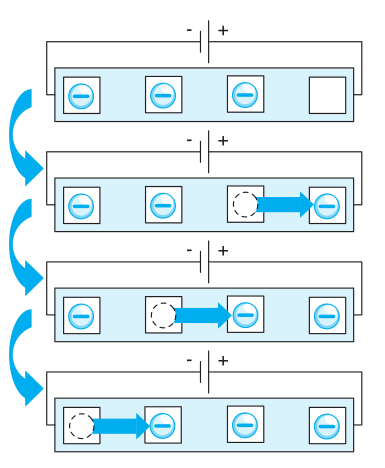
\includegraphics[scale=.4]{pictures/eigenleitung}
\end{figure}
\end{column}%
\end{columns}
\end{frame}


\begin{frame}{Elektronenüberschussleiter: $n$-Leiter}
\begin{columns}[T] % align columns
\begin{column}{.48\textwidth}
\begin{itemize}
	\item Struktur eines Elektronenüberschussleiters ($n$-Leiter)
	\item Einbau von Phosphoratomen zusätzliche Valenzelektronen im Gitter
	\item Zusätzliche Elektronen können sich nahezu ungehindert durch die Kristallstruktur bewegen
\end{itemize}
\end{column}%
\hfill%
\begin{column}{.48\textwidth}
\begin{figure}
\center
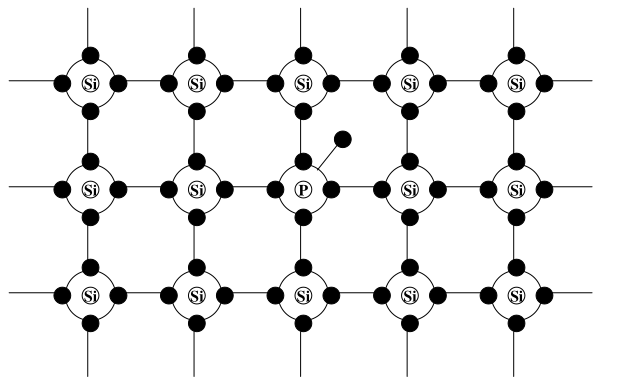
\includegraphics[scale=0.3]{pictures/n_leiter}
\end{figure}
\end{column}%
\end{columns}
\end{frame}

\begin{frame}{Elektronenmangelleiter: $p$-Leiter}
\begin{columns}[T] % align columns
\begin{column}{.48\textwidth}
\begin{itemize}
	\item Struktur eines Elektronenmangelleiters ($p$-Leiter)
	\item Einbau von Aluminiumatomen/Bohr entstehen künstliche Elektronenlöcher
	\item Elektronenlöcher wirken, wie positive Ladungsträger
\end{itemize}
\end{column}%
\hfill%
\begin{column}{.48\textwidth}
\begin{figure}
\center
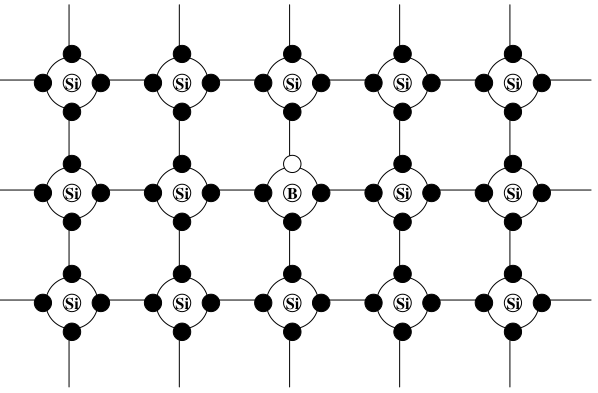
\includegraphics[scale=0.3]{pictures/p_leiter}
\end{figure}
\end{column}%
\end{columns}
\end{frame}

\section{Halbleiter}

\begin{frame}{Leiter/Halbleiter}
	\begin{itemize}
		\item Halbleiter sind Stoffe, deren elektrische Leitfähigkeit geringer als von\\
		Leitern und größer als von Nichtleitern sind
		\item Halbleiter wie Silizium und Germanium verfügen über eine Kristallstruktur
		\item Die Kristallstruktur wird mit hoher Reinheit hergestellt
		\item Auf ca. 1010 Atome kommt ein Fremdatom
		\item Die Eigenleitfähigkeit von Halbleitern basiert auf:
		\begin{itemize}
			\item Verunreinigung
			\item Aufbrechen von Kristallbindungen
			\item Oberflächen-Leitfähigkeit
		\end{itemize}

	\end{itemize}
\end{frame}

\subsection{Halbleiterdioden -- $pn$-Übergang}
\begin{frame}{Halbleiterdioden}
\begin{columns}[T] % align columns
\begin{column}{.48\textwidth}
\begin{itemize}
	\item Dioden: spezielle Schaltelemente
	\item Begrenzung des Stromfluss richtungsabhängig
	\item In Durchlassrichtung neutral
	\item In Sperrrichtung als Isolator
\end{itemize}
\end{column}%
\hfill%
\begin{column}{.48\textwidth}
\begin{figure}
\center
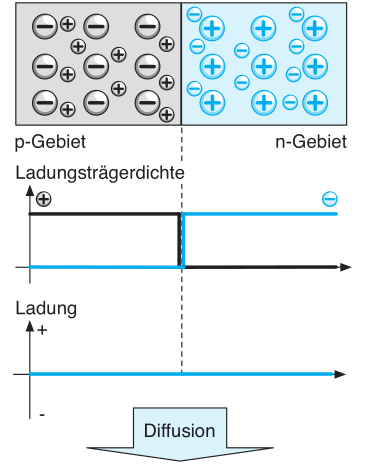
\includegraphics[scale=0.3]{pictures/halbleiterdiode1}
\end{figure}
\end{column}%
\end{columns}
\end{frame}

\begin{frame}{Halbleiterdioden -- $pn$-Übergang}
\begin{columns}[T] % align columns
\begin{column}{.48\textwidth}
\vspace*{0.5cm}
\begin{itemize}
	\item Dioden: spezielle Schaltelemente
	\item Begrenzung des Stromfluss richtungsabhängig
	\item In Durchlassrichtung neutral
	\item In Sperrrichtung als Isolator
\end{itemize}
\end{column}%
\hfill%
\begin{column}{.48\textwidth}
\begin{figure}
\center
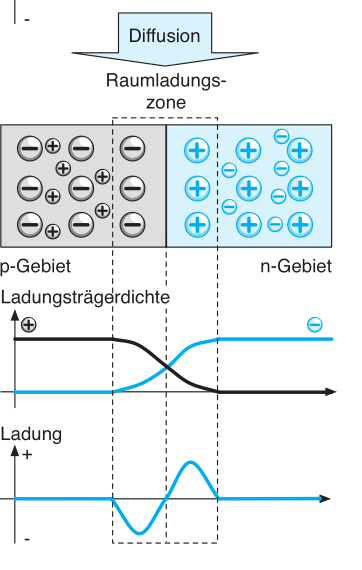
\includegraphics[scale=0.3]{pictures/halbleiterdiode2}
\end{figure}
\end{column}%
\end{columns}
\end{frame}

\begin{frame}{Halbleiterdioden -- $pn$-Übergang}
\begin{columns}[T] % align columns
\begin{column}{.48\textwidth}
\begin{itemize}
	\item Dioden: spezielle Schaltelemente
	\item Begrenzung des Stromfluss richtungsabhängig
	\item In Durchlassrichtung neutral
	\item In Sperrrichtung als Isolator
\end{itemize}
\end{column}%
\hfill%
\begin{column}{.48\textwidth}
\begin{figure}
\center
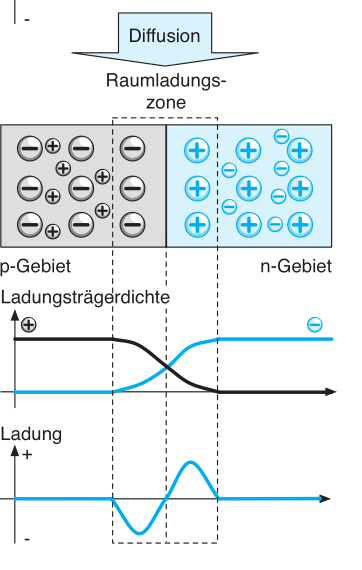
\includegraphics[scale=0.3]{pictures/halbleiterdiode2}
\end{figure}
\end{column}%
\end{columns}
\end{frame}

\begin{frame}{Halbleiterdioden -- $pn$-Übergang}
\begin{columns}[T] % align columns
\begin{column}{.48\textwidth}
\begin{itemize}
	\item Dioden: spezielle Schaltelemente
	\item Begrenzung des Stromfluss richtungsabhängig
	\item In Durchlassrichtung neutral
	\item In Sperrrichtung als Isolator
	\begin{itemize}
		\item Anlegen einer Spannung in Sperrrichtung
		\item Minuspol: $p$-Schicht, Pluspol $n$-Schicht
		\item Ladungsträger Richtung Spannungspole weggezogen
		\item D.h. Vergrößerung Sperrschicht $\to$ Isolator
	\end{itemize}
\end{itemize}
\end{column}%
\hfill%
\begin{column}{.48\textwidth}
\begin{figure}
\center
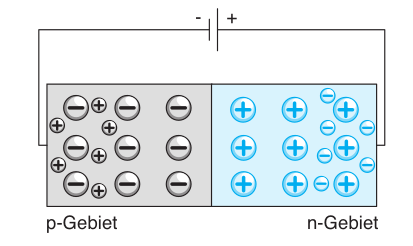
\includegraphics[scale=0.5]{pictures/sperrrichtung}
\end{figure}
\end{column}%
\end{columns}
\end{frame}

\begin{frame}{Halbleiterdioden -- $pn$-Übergang}
\begin{columns}[T] % align columns
\begin{column}{.48\textwidth}
\begin{itemize}
	\item Dioden: spezielle Schaltelemente
	\item Begrenzung des Stromfluss richtungsabhängig
	\item In Durchlassrichtung neutral
	\begin{itemize}
		\item Anlegen einer Spannung in Durchlassrichtung
		\item Minuspol: $n$-Schicht, Pluspol $p$-Schicht
		\item Freie Ladungsträger bewegen sich aufeinander zu
		\item D.h. Rekombination i.d. Sperrschicht $\to$ Leiter
	\end{itemize}
	\item In Sperrrichtung als Isolator
\end{itemize}
\end{column}%
\hfill%
\begin{column}{.48\textwidth}
\begin{figure}
\center
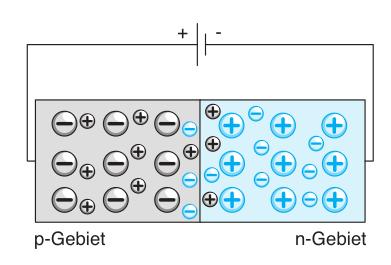
\includegraphics[scale=0.5]{pictures/durchlass}
\end{figure}
\end{column}%
\end{columns}
\end{frame}



\section{Transistor}
\begin{frame}{Transistor -- Transfer Resistor}
\begin{columns}[T] % align columns
\begin{column}{.48\textwidth}
	\begin{itemize}
		\item Gist: steuerbarer Widerstand
		\item Kann elektrisches Signal verstärken
		\item Digital ansteuerbar zum Ein- oder Ausschalten
		\item Bipolare Transistoren
		\begin{itemize}
			\item $npn$-Transistor
			\item $pnp$-Transistor
		\end{itemize}
		\item Unipolare Transistoren -- Feldeffekttransistor
		\begin{itemize}
			\item J-FET
			\item MOS-FET
		\end{itemize}
	\end{itemize}
\end{column}%
\hfill%
\begin{column}{.48\textwidth}
\begin{figure}
\center
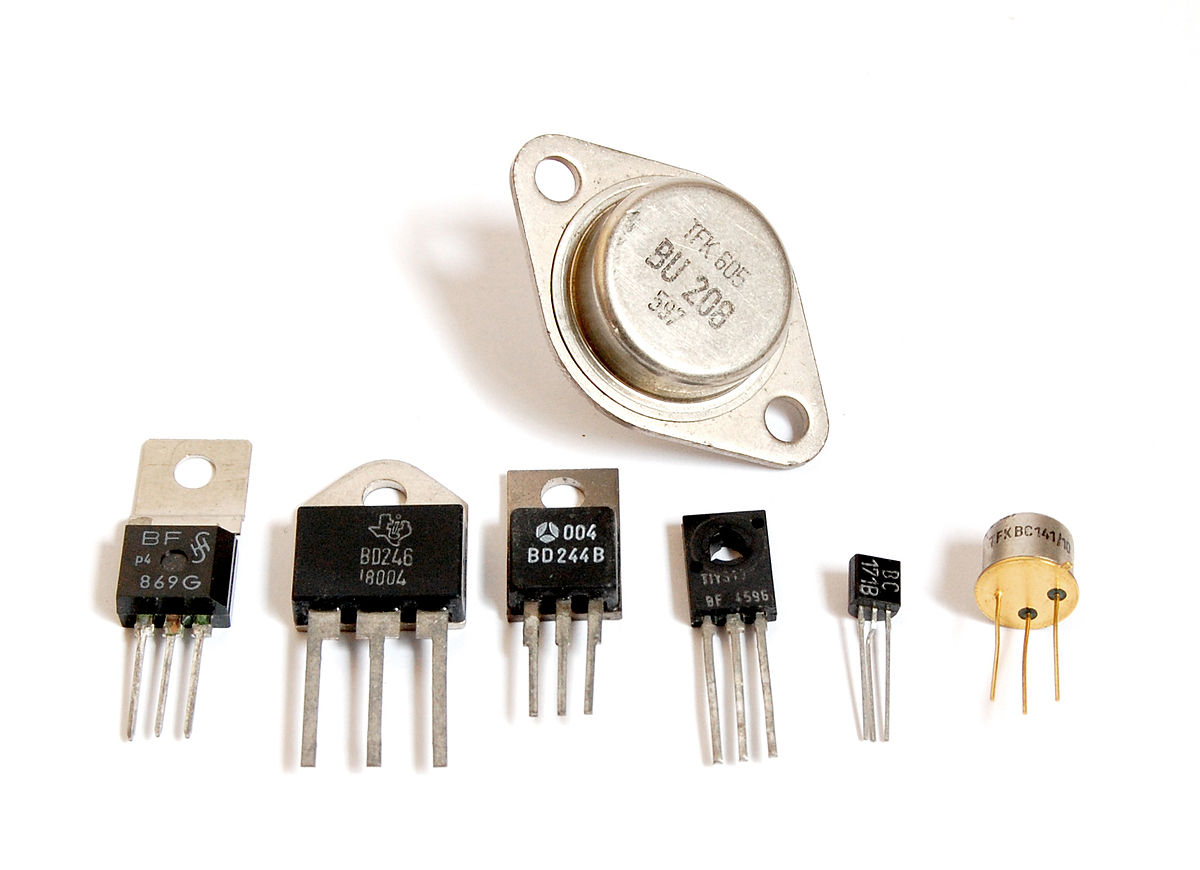
\includegraphics[scale=0.16]{pictures/transistors}
\end{figure}
\end{column}%
\end{columns}
\end{frame}

\subsection{npn-Transistor}
\begin{frame}{$npn$-Transistor}
\begin{columns}[T] % align columns
\begin{column}{.48\textwidth}
	\begin{itemize}
		\item Emitter \& Kollektor dienen Zufluss bzw. Abfluss der Elektronen
		\item Basis: Steueranschluss regelt den Stromfluss zwischen Emitter und Kollektor
		\item Steueranschluss verstärkende Wirkung:
		\begin{itemize}
			\item Geringe Änderung Stromfluss auf Emitter-Basis-Strecke
			\item $\to$ große Änderung des Stromflusses auf Emitter-Kollektor
		\end{itemize}
	\end{itemize}
\end{column}%
\hfill%
\begin{column}{.48\textwidth}
\begin{figure}
\center
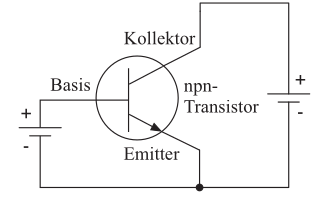
\includegraphics[scale=0.4]{pictures/npn_schema}\\
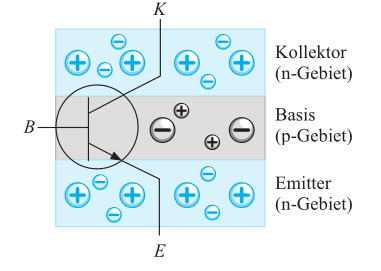
\includegraphics[scale=0.4]{pictures/npn_aufbau}
\end{figure}
\end{column}%
\end{columns}
\end{frame}

\begin{frame}{$npn$-Transistor: Basis-Emitter-Strecke}
\begin{columns}[T] % align columns
\begin{column}{.48\textwidth}
	\begin{itemize}
		\item $pn$-Übergang ist in Durchlassrichtung gepolt
		\item Ermöglicht in Abhängigkeit zur angelegten Spannung einen Stromfluss im Basisstromkreis
	\end{itemize}
\end{column}%
\hfill%
\begin{column}{.48\textwidth}
\begin{figure}
\center
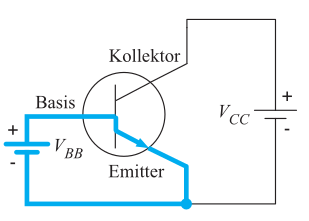
\includegraphics[scale=0.6]{pictures/be}
\end{figure}
\end{column}%
\end{columns}
\end{frame}

\begin{frame}{$npn$-Transistor: Basis-Kollektor-Strecke}
\begin{columns}[T] % align columns
\begin{column}{.48\textwidth}
	\begin{itemize}
		\item Basis besitzt gegenüber Kollektor negatives elektrisches Potenzial
		\item Stromfluss wird durch den in Sperrichtung gepolten $pn$-Übergang unterbunden
	\end{itemize}
\end{column}%
\hfill%
\begin{column}{.48\textwidth}
\begin{figure}
\center
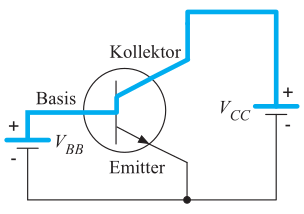
\includegraphics[scale=0.6]{pictures/bk}
\end{figure}
\end{column}%
\end{columns}
\end{frame}

\begin{frame}{$npn$-Transistor: Emitter-Kollektor-Strecke}
\begin{columns}[T] % align columns
\begin{column}{.48\textwidth}
	\begin{itemize}
		\item Zwischen Emitter und Kollektor stellt sich ein Stromfluss ein
		\item Stärke proportional mit der Stärke des Basisstroms zunimmt
	\end{itemize}
\end{column}%
\hfill%
\begin{column}{.48\textwidth}
\begin{figure}
\center
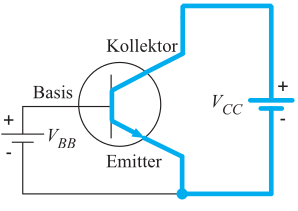
\includegraphics[scale=0.6]{pictures/ek}
\end{figure}
\end{column}%
\end{columns}
\end{frame}

\begin{frame}{$pnp$-Transistor: Emitter-Kollektor-Strecke}
\begin{columns}[T] % align columns
\begin{column}{.58\textwidth}
	\begin{itemize}
		\item Zusammensetzung der Halbleiter \enquote{invers} zu $pnp$
		\item Basis $n$-Gebiet
		\item Emitter und Kollektor dagegen $p$-Gebiet
		\item Positive Spannung am Emitter eine Flut von Elektronenlöchern aus dem $p$-Leiter in das $n$-Gebie
		\item Negative Spannung	: fließt geringer Teil der Defektelektronen über Basis ab
		\item Großteil der Elektronenlöcher wird durch die starke negative Kollektorspannung in die obere $p$-Schicht gezogen
		\item $\to$ fließt als Kollektorenstrom ab
	\end{itemize}
\end{column}%
\hfill%
\begin{column}{.38\textwidth}
\begin{figure}
\center
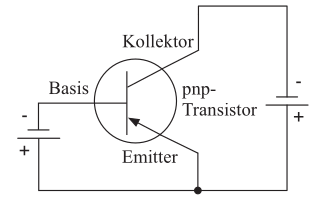
\includegraphics[scale=0.4]{pictures/pnp_schema}\\
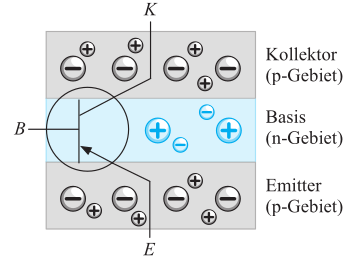
\includegraphics[scale=0.4]{pictures/pnp_aufbau}
\end{figure}
\end{column}%
\end{columns}
\end{frame}

\subsection{Schaltungen mit npn-Transistor}
\begin{frame}{Buffer-Schaltungen mit $npn$-Transistor}
\begin{figure}
\center
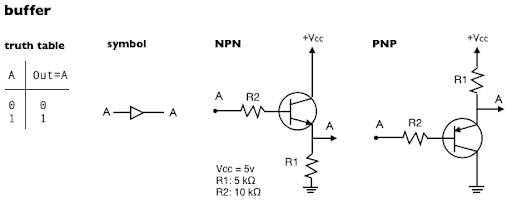
\includegraphics[scale=0.8]{pictures/buffer}
\end{figure}
\end{frame}


\begin{frame}{Not-Schaltungen mit $npn$-Transistor}
\begin{figure}
\center
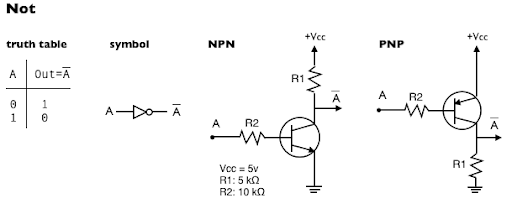
\includegraphics[scale=0.8]{pictures/not}
\end{figure}
\end{frame}


\begin{frame}{AND-Schaltungen mit $npn$-Transistor}
\begin{figure}
\center
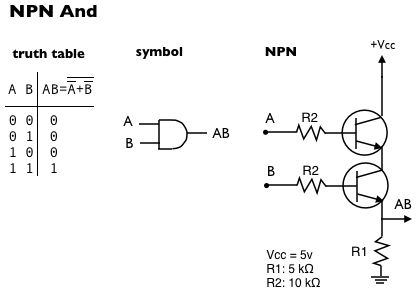
\includegraphics[scale=0.65]{pictures/and}
\end{figure}
\end{frame}

\begin{frame}{NAND-Schaltungen mit $npn$-Transistor}
\begin{figure}
\center
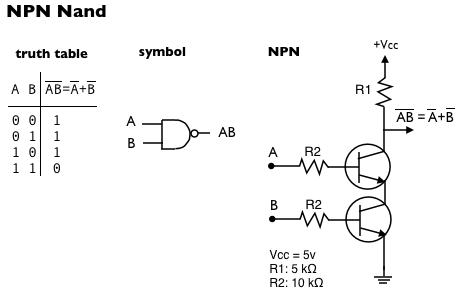
\includegraphics[scale=0.65]{pictures/nand}
\end{figure}
\end{frame}


\begin{frame}{OR-Schaltungen mit $npn$-Transistor}
\begin{figure}
\center
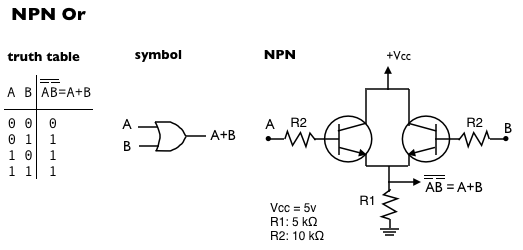
\includegraphics[scale=0.6]{pictures/or}
\end{figure}
\end{frame}

\begin{frame}{NOR-Schaltungen mit $npn$-Transistor}
\begin{figure}
\center
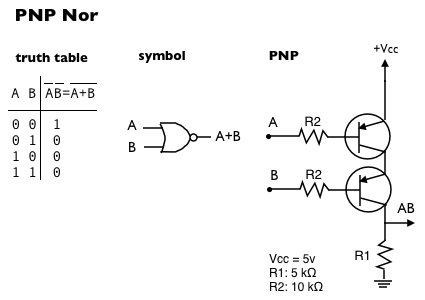
\includegraphics[scale=0.65]{pictures/nor}
\end{figure}
\end{frame}

\section*{Quellen}
\appendix
\begin{frame}[allowframebreaks]
  \frametitle<presentation>{Quellen}
\printbibliography
\end{frame}
\end{document}